\hoofdstuk{Introduction}

\paragraaf{Problem statement}

Lunatech has demand for the development of cross-platform mobile applications. Currently these applications are bening developed using webtechnologies such as HTML5 and Javascript. A mobile application developed this way is refered to as webapp because it runs in a browserbased environment and is often hosted at a webserver rather than downloaded to the device itself.
%\footnote{Note: when mentioning the word 'current', it refers to the old situation as the process to get to the actual current situation is being illustrated}

The problem with webapps is that they lack in user experience. This is mainly due manner in which user interface components are build in HTML. Every platform has its own set of recognizable elements, but these cannot be accessed from within the browser environment. As a result of this the app will feel dislocated to the user because it's style doesn't match the rest of the platform. It tries to look and feels native, but never gets arround the fact that it's a webapp.

The direct alternative to webapps are native apps, native are writting using technologies proprietary to each platform, hench the term 'native'. What these applications lose in terms of cross-platform support they make up in terms of user experience.  A native apps has acces to all the platforms propietary libraries and can rely on the user interface elements provided through these libraries.

Lunatech would like to know how to make use of the look-and-feel from native apps with the cross-platform support of webapps.

\paragraaf{Research questions}

Main research question:
\begin{itemize}
\item \emph{How to develop a cross-platform mobile application while retaining the native look-and-feel?}
\end{itemize}

\noindent Sub research questions:
\begin{itemize}
% \item \emph{Which mobile platforms should be targetted for cross-platform mobile application development?}
% \item \emph{How is the native look-and-feel defined?}
\item \emph{Is it viable to implement a custom solution to cross-platform mobile application development?}
\item \emph{Which solutions to cross-platform mobile application development currently exist?}
\item \emph{Which of these solutions offer the defined native look-and-feel?}
\item \emph{Are these solutions viable for commerical useage?}
\end{itemize}

\paragraaf{Research method}

This paragraph will describe the method used during the research.\\

First the context of the main research question needs to be determined by defining the concepts \emph{native look-and-feel} and \emph{cross-platform}. The \emph{native look-and-feel} is defined by the a set of criteria related to the user experience while \emph{cross-platform} is defined by determining which platforms should be targetted.

% Once the concepts in main research question are fully defined the possiblity to look for existing solutions opens up.

% First the \emph{native look-and-feel} needs to be defined. After which it's nessecary to define the scope of \emph{cross-platform} by determining which platforms should be targetted.

Once the concepts in main research question are defined it is needed to research which solutions which fit within the context. During a preliminary research a market survey will have to be performed in order to deterime which solutions to cross-platform app development are available on todays market. Each found solution will be given a closer look and categorized based on requirements provided by Lunatech. Once the categorization is complete the solutions will be filtered based on how far the requirements have been met.

A comparisson test will be performed in order to determine which solution meets is potentially viable for commercial use by Lunatech. This test will consist of a short analysis per solution based on by Lunatech criteria, and a practical part where a benchmark application will be built. The results will be compared and the solution which offers the most complete set of features will be deemed potentially viable for commercial use by Lunatech. At this point a decision has to be made whether to continue with the potentially viable existing solution or research a custom solution. 

To determine if the chosen solution is viable for commercial use by Lunatech a case study will be performed based on a realistic scenario Lunatech might encounter. During this case study the solution will be analysed and evaluated.

The results of the case study and the analysis will participate to answering how to develop a cross-platform mobile application while retaining the native look-and-feel. In addition to answering the main research question an recommendation will be given to Lunatech regarding the possible adoptation of the solution for commercial usage.

%todo methode verantwoording.

\newpage
\begin{centering}
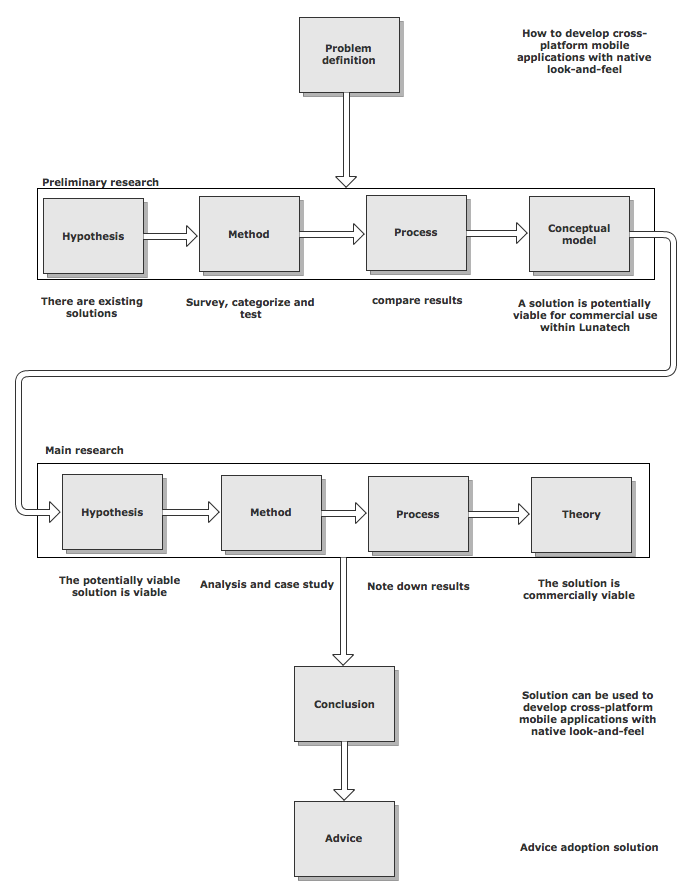
\includegraphics[scale=0.6]{images/researchprocess.png}\\{Research method diagram}\\
\end{centering}

%verantwoorden: why it works analysis. + verantwoorden niet naar andere oplossingen kijken.

